%!TEX TS-program = xelatex
%!TEX encoding = UTF-8 Unicode
% Awesome CV LaTeX Template for Cover Letter
%
% This template has been downloaded from:
% https://github.com/posquit0/Awesome-CV
%
% Authors:
% Claud D. Park <posquit0.bj@gmail.com>
% Lars Richter <mail@ayeks.de>
%
% Template license:
% CC BY-SA 4.0 (https://creativecommons.org/licenses/by-sa/4.0/)
%



%-------------------------------------------------------------------------------

% Color for highlights
% Awesome Colors: awesome-emerald, awesome-skyblue, awesome-red, awesome-pink, awesome-orange
%                 awesome-nephritis, awesome-concrete, awesome-darknight


%-------------------------------------------------------------------------------
% CONFIGURATIONS
%-------------------------------------------------------------------------------
% A4 paper size by default, use 'letterpaper' for US letter
\documentclass[11pt, a4paper]{awesome-cv}

% Configure page margins with geometry
\geometry{left=1.4cm, top=.8cm, right=1.4cm, bottom=1.8cm, footskip=.5cm}

% Specify the location of the included fonts
\fontdir[fonts]
 
% \definecolor{lighttext}{HTML}{CA63A8}

% Set false if you don't want to highlight section with awesome color

% If you would like to change the social information separator from a pipe (|) to something else
\renewcommand{\acvHeaderSocialSep}{\quad\textbar\quad}


\colorlet{awesome}{awesome-red}

% Uncomment if you would like to specify your own color
% \definecolor{awesome}{HTML}{CA63A8}

% Colors for text
% Uncomment if you would like to specify your own color
% \definecolor{darktext}{HTML}{414141}
% \definecolor{text}{HTML}{333333}
% \definecolor{graytext}{HTML}{5D5D5D}
% \definecolor{lighttext}{HTML}{999999}

% Set false if you don't want to highlight section with awesome color
 % Colors for text
% Uncomment if you would like to specify your own color
 \definecolor{darktext}{HTML}{000000}
 \definecolor{text}{HTML}{000000}
 \definecolor{graytext}{HTML}{000000}
 \definecolor{lighttext}{HTML}{000000}
 
 
 \setbool{acvSectionColorHighlight}{true}

 

 
 
 
%-------------------------------------------------------------------------------
%	PERSONAL INFORMATION
%	Comment any of the lines below if they are not required
%-------------------------------------------------------------------------------
% Available options: circle|rectangle,edge/noedge,left/right
%\photo{2020-01-18.jpg}
\name{Ismail}{EZZAKI}
\position{Master Student{\enskip\cdotp\enskip}Freelancer Programmer}
\address{812 Ait kdif Ouarzazate Morocco}

\mobile{(+212) 708070221}
\email{ismail.ezzaki@edu.uca.ma}
\homepage{ismailezzaki.me}
\github{ismailezzaki96}
% \gitlab{gitlab-id}
% \stackoverflow{SO-id}{SO-name}
% \twitter{@twit}
% \skype{skype-id}
% \reddit{reddit-id}
% \medium{madium-id}
% \googlescholar{googlescholar-id}{name-to-display}
%% \firstname and \lastname will be used
% \googlescholar{googlescholar-id}{}
% \extrainfo{extra informations}

\quote{``be the change you want to see in the world"}

%-------------------------------------------------------------------------------
%	LETTER INFORMATION
%	All of the below lines must be filled out
%-------------------------------------------------------------------------------
% The company being applied to
\recipient
 {Company Recruitment Team}
 {Google Inc.\\1600 Amphitheatre Parkway\\Mountain View, CA 94043}
% The date on the letter, default is the date of compilation
\letterdate{\today}
% The title of the letter
\lettertitle{Statement of Research Interests}
% How the letter is opened
\letteropening{}
\newcommand{\thesis}{ position in experimental neutrino physics
}

% How the letter is closed
\letterclosing{Sincerely,}
% Any enclosures with the letter
\letterenclosure[Attached]{Curriculum Vitae}


%-------------------------------------------------------------------------------
\begin{document}

% Print the header with above personal informations
% Give optional argument to change alignment(C: center, L: left, R: right)
%\makecvheader[C]

% Print the footer with 3 arguments(<left>, <center>, <right>)
% Leave any of these blank if they are not needed

% Print the title with above letter informations
\makelettertitle




%-------------------------------------------------------------------------------
%	LETTER CONTENT
%-------------------------------------------------------------------------------
\begin{cvletter}
 \lettersection{Research Area and Approach }

My primary field of research interest is computational physics. More precisely, I am interested in problems related to particle physics. 

Because of the intrinsic interdisciplinary nature of computational physics, my interests often overlap with other areas of computer science such as machine learning, algorithms, and data analysis. 

In the following, I will briefly summarize some of my research projects related to computational and particle physics.

 \lettersection{Current and Past Research }
\textbf{Generative Adversarial Networks to simulate events in ATLAS experiment (duration: 3 months) 
}\\
I investigate the possibility of using Generative Adversarial Networks as a tool to create analysis-specific datasets for LHC data analyses. 

I apply this idea to the generation of muon four-momenta in Z → μμ events at the Atlas experiment. I generate the dataset with PYTHIA and Delphes and use the promising performances of GANs to learn complicated probability distribution functions.

Based on the KS test, I propose an objective criterion to select the best model in a quantitative way, i.e., not just relying on a qualitative by-eye assessment of the generator performance. 

\textbf{\color{blue} results obtained: }

\begin{figure*}[h]
	\centering
	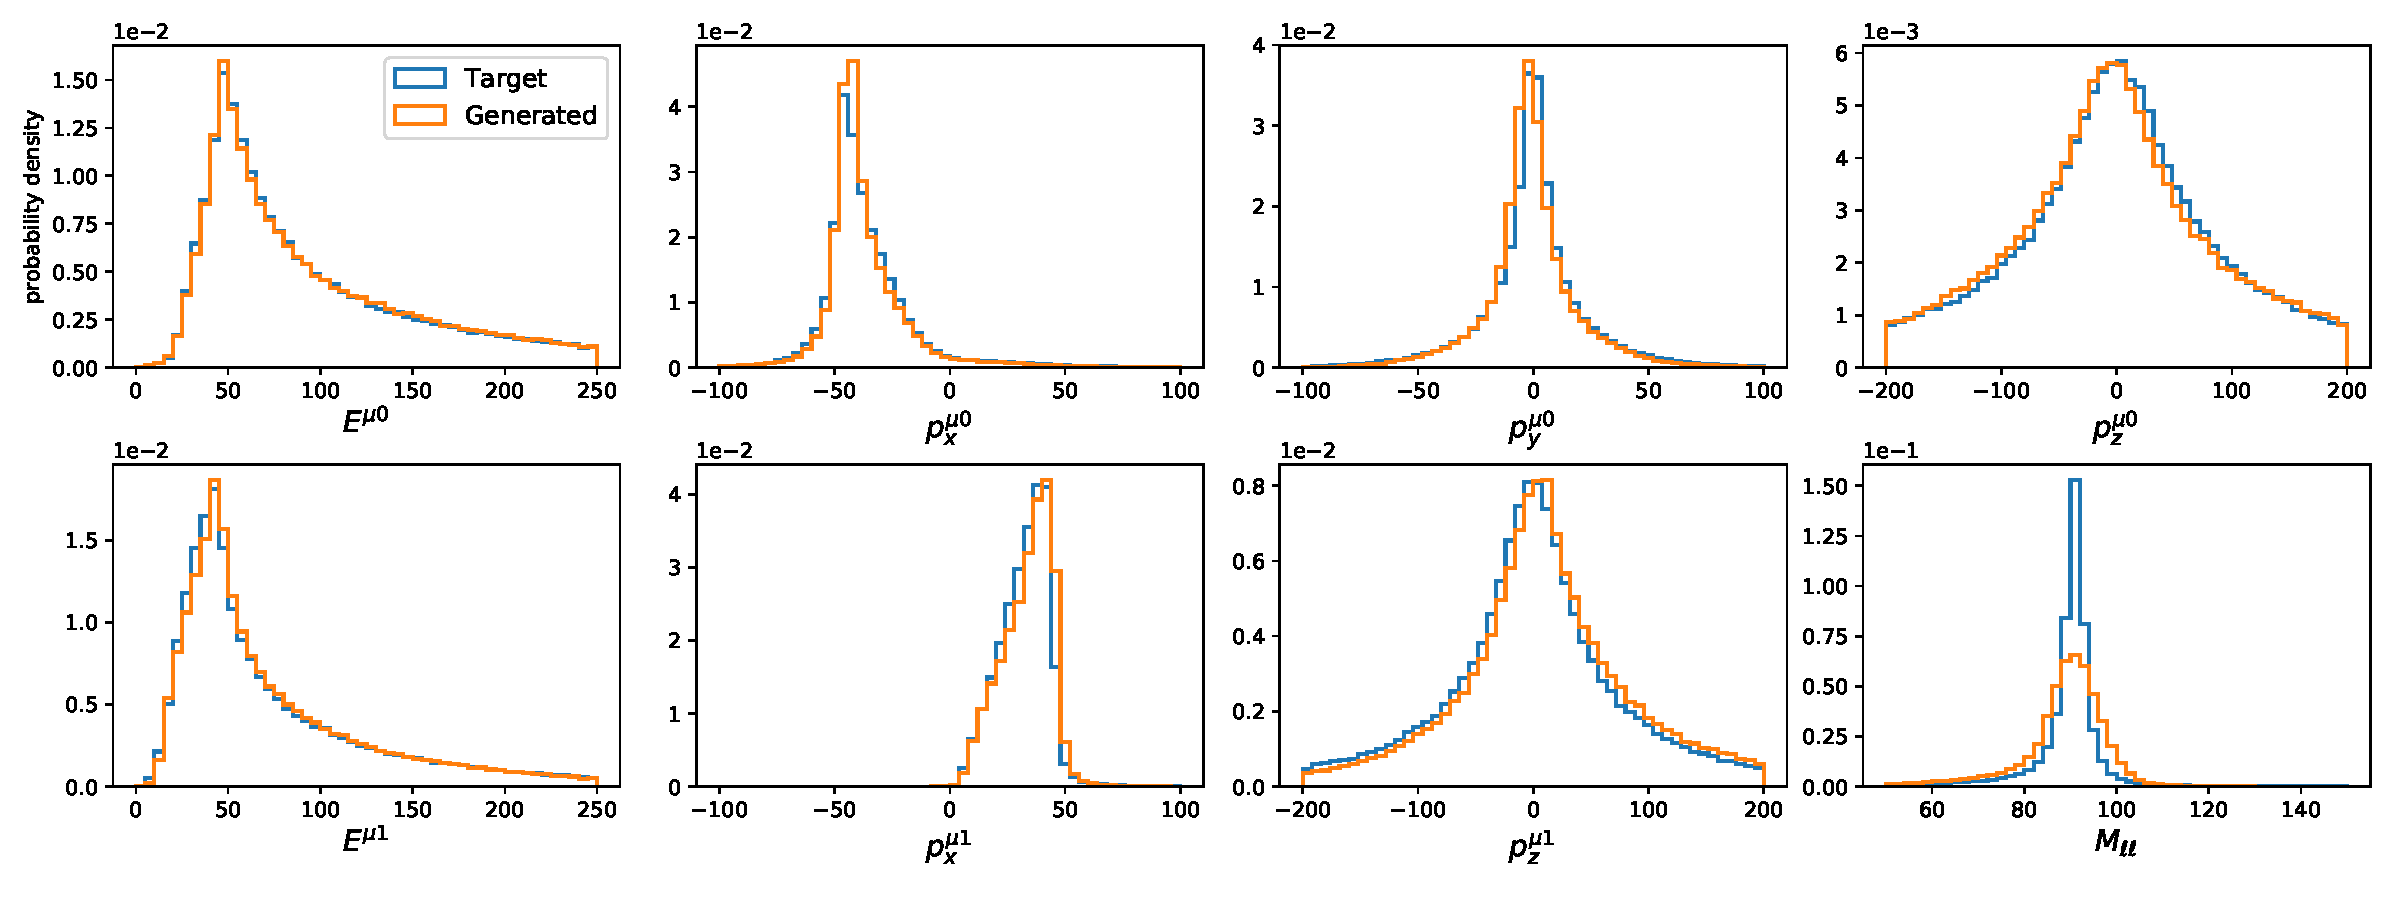
\includegraphics[width=\textwidth]{figs/trial3_epoch39200_minigantest_final.pdf}
\end{figure*}
The biggest upside of this method would be that datasets derived in this manner will be analysis-specific. On one hand, this would reduce the amount of MC to be centrally produced, also allowing to reduce the intermediate storage utilization. On the other hand, each analysis will require a dedicated training and a dedicated output dataset. 


In my opinion, Generative models could instead be used to augment statistics for the largest samples, reducing the need for full simulation, generating the target dataset with PYTHIA and Delphes was found to be $\sim$ 3600 times slower; the generator model is stored in a file that is smaller than 10 MBs, whereas the generated events take up 2 GBs, a reduction of two orders of magnitude in size. 

 
 \newpage
\textbf{Simulation of a Mach Zehnder interferometer as a coronagraph (duration: 1 month) 
}\\
Our laboratory controls the Oukaimeden observatory in Marrakech and I collaborated with another master student in astrophysics to simulate the image results for a telescope that uses a Mach-Zehnder interferometer as a coronagraph 

The goal of this simulation is to help us to quickly get an idea of what we can see through an instrument that uses this technology 

The coronagraph acts as a frequency filter. The major advantage of the coronagraph is to reduce the light of a central star to improve the contrast of its faint companions so we can observe it  

Despite my low knowledge of adaptive optics, I could create the simulation based on the mathematical model and physics properties of the instrument. We develop the simulation using Python and we built the graphic interface using Tkinter 


\textbf{\color{blue} the mathematical model: }

\begin{figure*}[h]
	\centering
	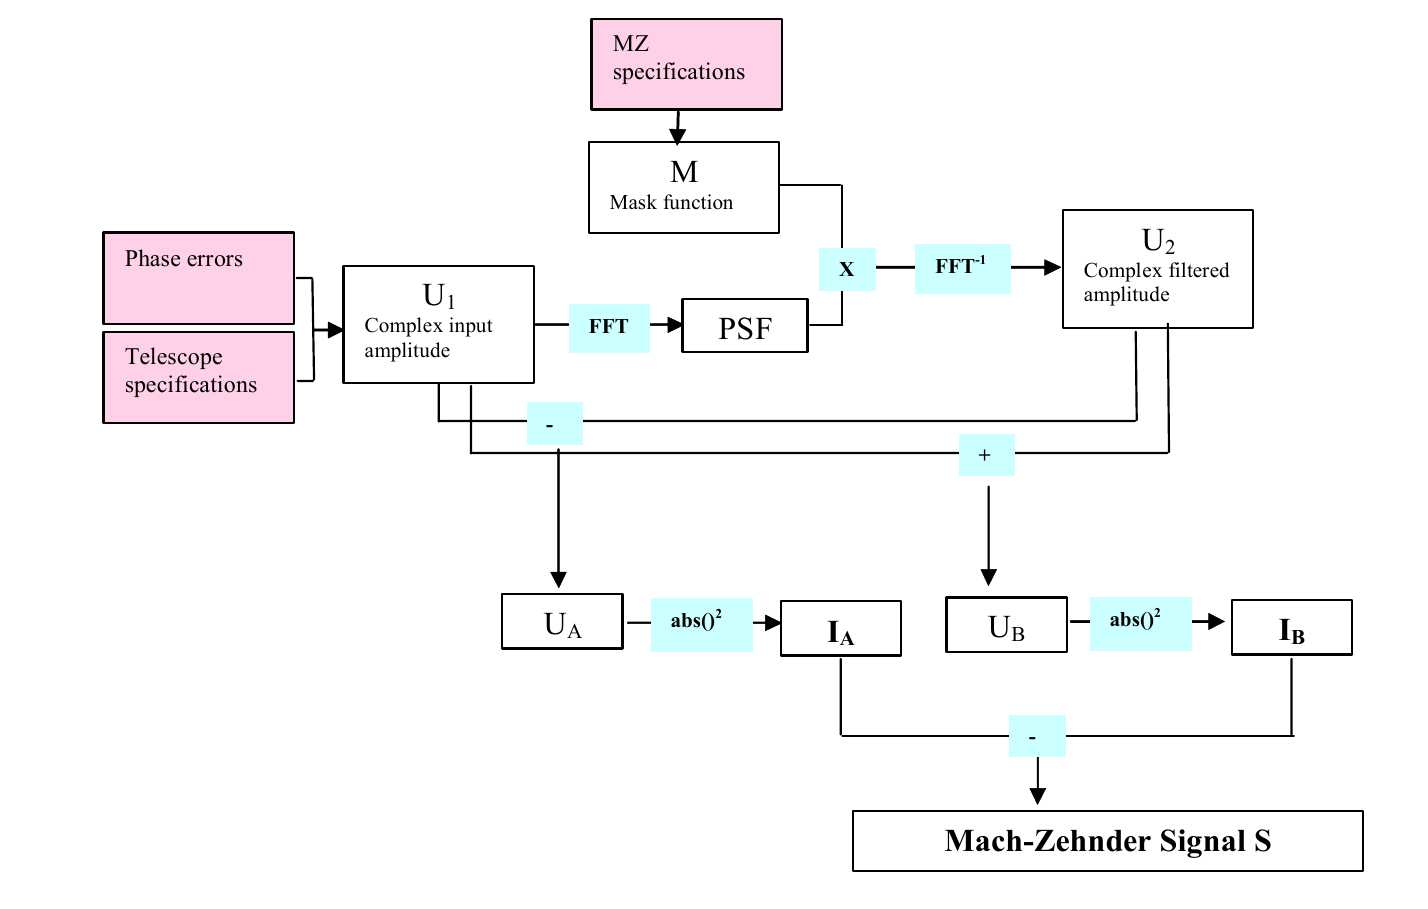
\includegraphics[width=0.6\textwidth]{figs/svg.png}
\end{figure*}

\textbf{Master Thesis (duration: 4 months) 
}

Unfortunately, because of the COVID-19 lockdown, my master internship in germany was canceled, and it forced me to do my master thesis on a subject far from my interest in particle physics 

My master thesis was about black hole thermodynamics and phase transition 

The computational part of my master thesis comprises developing a script in python and Mathematica to:  

\begin{itemize}
\item Find and draw programmatically the shape of famous space-time types spacetime in different coordinate system 
\item calculate the thermodynamics properties for the four genaral black holes types  
\item Find programmatically the analytical expression of every critical point and the associated phase transitions for all these black holes : these calculations were done by Sagemath Library and Sympy in python 
\end{itemize}



\lettersection{Future Research Directions}
As regards my future physics interests, I would like to continue in computational physics and made more software that make the life of physicist easier, also after my experience with machine learning, I want to focus on the usage of its features in my programs since it is quickly providing new powerful tools for physicists either in experiments or simulations. 


\end{cvletter}


%-------------------------------------------------------------------------------
% Print the signature and enclosures with above letter informations

\end{document}
